%%
%% SENTINEL: LSM-eBPF Co-Design with Intent Provenance Graphs and Dual-Tier
%%           Local LLM Inference for Confidence-Weighted APT Enforcement
%%
%% Submitted to: IEEE Transactions on Information Forensics and Security (TIFS)
%% Template:     IEEEtran (journal style)
%%

\documentclass[journal]{IEEEtran}

\linespread{0.95}

%% ── Packages ──────────────────────────────────────────────────────────────────
%% xcolor must be loaded first (with options) before tikz/listings pull it in
\usepackage[dvipsnames,table]{xcolor}
\usepackage[T1]{fontenc}
\usepackage{amsmath,amssymb,amsthm}
\usepackage{graphicx}
\usepackage{tikz}
\usetikzlibrary{arrows.meta,positioning,shapes.geometric,shapes.misc,fit,
                backgrounds,calc,decorations.pathreplacing,matrix,shadows}
\usepackage{pgfplots}
\pgfplotsset{compat=1.18}
\usepackage{booktabs}
\usepackage{multirow}
\usepackage{algorithm}
\usepackage{algpseudocode}
\usepackage{listings}
\usepackage{cite}
\usepackage{url}
\usepackage{microtype}
\usepackage{balance}
\usepackage{placeins}
\usepackage{orcidlink}  % hyperlinked ORCID logo; set \AuthorOrcid below
\usepackage{hyperref}
\hypersetup{colorlinks=false,pdfborder={0 0 0},hidelinks}

%% Author ORCID — register free at https://orcid.org/register, then paste digits only:
%% Example: \renewcommand{\AuthorOrcid}{0000-0002-1234-5678}
\newcommand{\AuthorOrcid}{0009-0003-7291-360X}

\setlength{\textfloatsep}{8pt plus 2pt minus 2pt}
\setlength{\floatsep}{6pt plus 2pt minus 2pt}
\setlength{\intextsep}{6pt plus 2pt minus 2pt}
\setlength{\dbltextfloatsep}{8pt plus 2pt minus 2pt}
\setlength{\dblfloatsep}{6pt plus 2pt minus 2pt}

%% ── Listings style ────────────────────────────────────────────────────────────
\definecolor{codebg}{rgb}{0.97,0.97,0.97}
\definecolor{codekey}{rgb}{0.0,0.3,0.6}
\definecolor{codecomment}{rgb}{0.3,0.5,0.3}
\lstset{
  backgroundcolor=\color{codebg},
  basicstyle=\ttfamily\tiny,
  keywordstyle=\color{codekey}\bfseries,
  commentstyle=\color{codecomment}\itshape,
  breaklines=true,
  frame=single,
  numbers=left,
  numberstyle=\tiny\color{gray},
  xleftmargin=1.5em,
  framexleftmargin=1.5em,
  captionpos=b
}

%% ── Theorem environments ──────────────────────────────────────────────────────
\newtheorem{definition}{Definition}
\newtheorem{theorem}{Theorem}
\newtheorem{proposition}{Proposition}
\newtheorem{lemma}{Lemma}
\newtheorem{hypothesis}{Hypothesis}

%% ── Macros ───────────────────────────────────────────────────────────────────
\newcommand{\sentinel}{\textsc{Sentinel}}
\newcommand{\ipg}{IPG}
\newcommand{\cwae}{CWAE}
\newcommand{\ebpf}{eBPF}
\newcommand{\ie}{\textit{i.e.}}
\newcommand{\eg}{\textit{e.g.}}
\newcommand{\etal}{\textit{et al.}}

%% ─────────────────────────────────────────────────────────────────────────────
\begin{document}

\title{SENTINEL: LSM-eBPF Co-Design with Graph-Structured LLM Inference\\
for Zero-Trust APT Detection}

\author{%
  \IEEEauthorblockN{Juharasha Shaik%
    \ifx\AuthorOrcid\empty\else\,\orcidlink{\AuthorOrcid}\fi}
  \IEEEauthorblockA{\textit{Independent Researcher}\\
                    Fremont, CA 94538, USA\\
                    Email: shaik.juharasha@gmail.com%
                    \ifx\AuthorOrcid\empty\else\\ORCID: \url{https://orcid.org/\AuthorOrcid}\fi}
  \thanks{Manuscript received June 08, 2026.
  The author received no external funding for this work.
  (\emph{Corresponding author}: Juharasha Shaik, shaik.juharasha@gmail.com.)}}

\maketitle

%% ─────────────────────────────────────────────────────────────────────────────
\begin{abstract}
Contemporary host-based intrusion detection systems (HIDS) suffer from a
critical semantic gap: they observe \emph{what} a process does but cannot
reason about \emph{why} it does so.  Rule-based eBPF engines such as Falco
attach to tracepoints that fire \emph{before} the kernel resolves the final
object, leaving them vulnerable to time-of-check-to-time-of-use (TOCTOU)
races and path-aliasing attacks. We present \sentinel{}, an IPG-centric
forensic architecture that addresses these limitations by utilizing an
Intent Provenance Graph (\ipg{}) as a unified intermediate representation (IR)
for host-level activity. A deterministic \texttt{provenance\_score()} graph
scorer acts as the primary detector; a local LLM classifies gray-zone windows
($0.15 < g < 0.55$) and produces MITRE ATT\&CK attribution, while clear
benign/malicious windows bypass LLM inference. CoVe-verified LLM outputs and an
LTL symbolic guardian enforce hard safety floors and prevent evasions.
Evaluated on DARPA TC~E3 CADETS, hybrid graph-first fusion achieves behavioral-only
F1\,$=$\,0.603 (LLM-only v4: 0.597) and TI-aided F1\,$=$\,0.915; on a 15-trace
attack strace subset, \ipg{} reduces tokens by 57.5\% at window size~20 (83.3\% full trace)
using local Ollama Llama-3.1-8B without cloud dependence.
\end{abstract}

\begin{IEEEkeywords}
eBPF, LSM hooks, TOCTOU-resistant security, zero-trust enforcement,
intent provenance graphs, graph-structured prompting, large language models,
SSL/TLS uprobe, AI agent monitoring, host-based intrusion detection,
confidence-weighted adaptive enforcement, chain of verification,
LTL symbolic guardian, program-counter-aware behavioral provenance,
process injection detection, APT detection.
\end{IEEEkeywords}

%% ═════════════════════════════════════════════════════════════════════════════
\section{Introduction}\label{sec:intro}
%% ═════════════════════════════════════════════════════════════════════════════

The modern threat landscape is dominated by Advanced Persistent Threats (APTs)
that evade signature-based detection by employing \emph{living-off-the-land}
(LotL) tactics---abusing trusted system utilities (\eg{} \texttt{bash},
\texttt{curl}, \texttt{python3}) to blend attack traffic with legitimate
behavior~\cite{darpa_tc}.  In these scenarios, no individual system call
is inherently malicious; only the \emph{causal sequence and context} reveal
attacker intent.

Traditional HIDS such as OSSEC~\cite{ossec} and Tripwire rely on file
integrity checks and static rule sets that are both brittle (high false
negatives against novel techniques) and slow (polling-based, high overhead).
eBPF-based rule engines such as Falco~\cite{falco} and
Tetragon~\cite{tetragon} improve performance by executing in the kernel, but
their expressiveness is bounded by manually authored rules---a fundamental
limitation against zero-day and polymorphic attacks.
Deep learning detectors such as DeepLog~\cite{deeplog} and
LogBERT~\cite{logbert} achieve higher semantic coverage but require
significant GPU resources, offline training phases, and lack the ability to
\emph{block} an ongoing attack in real time.

The confluence of three recent advances creates a new design space.
\emph{eBPF LSM hooks}~\cite{bpf_lsm_kernel} fire \emph{after} the kernel
resolves the true object identity, eliminating TOCTOU vulnerabilities inherent
to tracepoint-based detectors used by all prior eBPF tools.
\emph{Quantized local LLMs} (\eg{} Llama-3-8B-GGUF~\cite{llama3}) run on
commodity x86 Linux via local Ollama (CPU or optional GPU acceleration),
enabling semantic reasoning without external API calls.
\emph{eBPF uprobes} on TLS library functions expose decrypted AI agent traffic,
opening a new monitoring surface for prompt-injection-driven attacks.
Combining all three, however, is non-trivial:

\begin{itemize}
  \item \textbf{TOCTOU exposure}: All published eBPF detectors attach to
        \texttt{sys\_enter\_*} tracepoints, which fire before the kernel
        resolves symlinks and bind mounts, enabling path-substitution evasion.
  \item \textbf{Token efficiency}: Naïve serialization of a 20-event syscall
        window consumes $\sim$850 LLM tokens per process, making real-time
        multi-process monitoring prohibitively expensive.
  \item \textbf{Invocation rate}: A lightly loaded server generates
        $\sim$3{,}000 syscalls/second; submitting every window to an LLM is
        computationally infeasible.
  \item \textbf{Enforcement granularity}: Binary block/allow decisions
        (Falco, Tetragon) miss the nuanced spectrum between a suspicious but
        uncertain event and a high-confidence ongoing attack.
  \item \textbf{AI agent blind spot}: Autonomous AI agents (Claude Code,
        Copilot Workspace, AutoGPT) execute shell commands via TLS-encrypted
        API calls invisible to syscall-only monitors.
\end{itemize}

\vspace{2pt}
\noindent\textbf{Contributions.} This paper makes the following original
contributions:

\begin{enumerate}
  \item \textbf{LSM-eBPF Co-Design for TOCTOU-Resistant Telemetry}: We replace
        tracepoints with BPF LSM hooks (\texttt{lsm/bprm\_check\_security},
        \texttt{lsm/file\_open}, \texttt{lsm/socket\_connect}) available since
        Linux~5.7. These hooks fire post-resolution, closing the structural
        TOCTOU window available to tracepoint-based eBPF detectors at hook time
        (Section~\ref{sec:lsm}; measured race discrepancy in \S\ref{sec:eval_lsm}).
  \item \textbf{Intent Provenance Graph (IPG) Serialization}: A directed multigraph
        encodes causal syscall structure, reducing token consumption by 57.5\% at window size 20
        and 83.3\% on full traces (measured with tiktoken on 15 GCP-captured strace files, 5 attack
        traces averaged at $n{=}20$), and is
        serialized as structured YAML for LLM input (Section~\ref{sec:ipg}).
  \item \textbf{Hybrid Graph-First Inference Pipeline}: We design a graph-first detection
        architecture where a deterministic graph scorer acts as the primary filter, and a local
        LLM is reserved as an escalation path for gray-zone events (Section~\ref{sec:pipeline}).
  \item \textbf{Hybrid Safety Floors (LTL Guardian \& PCABP)}: We combine a Linear Temporal Logic
        (LTL) Symbolic Guardian to enforce formal safety axioms with Program-Counter-Aware Behavioral
        Provenance (PCABP) address-space tracing to prevent evasion attacks and enforce deterministic
        policy limits (Section~\ref{sec:ltl}, Section~\ref{sec:pcabp}).
  \item \textbf{Confidence-Weighted Adaptive Enforcement (CWAE) \& Chain of Verification (CoVe)}:
        We present a multi-tier enforcement engine (CWAE) and a 4-step grounding loop (CoVe) that fuses
        graph scores, LLM confidence, and LTL violations to compute unified enforcement tiers (Section~\ref{sec:enforce}, Section~\ref{sec:cove}).
\end{enumerate}

\noindent The full async Python implementation, Docker deployment, MITRE
ATT\&CK simulation suite, captured strace corpora, and all evaluation
scripts are publicly available at
\url{https://github.com/jshaik-lab/ebpf-lsm-apt-monitor}
(see Data Availability Statement for dataset and Zenodo DOI details).

The remainder reviews related work (Section~\ref{sec:background}), threat model
(Section~\ref{sec:threat}), architecture (Section~\ref{sec:design}),
implementation (Section~\ref{sec:impl}), evaluation (Section~\ref{sec:eval}),
security analysis (Section~\ref{sec:analysis}), and conclusion
(Section~\ref{sec:conclusion}).

%% ═════════════════════════════════════════════════════════════════════════════
\section{Background and Related Work}\label{sec:background}

Prior eBPF HIDS (Falco~\cite{falco}, Tetragon~\cite{tetragon}) attach to
\texttt{sys\_enter\_*} tracepoints \emph{before} object resolution, enabling
TOCTOU evasion; BPF~LSM~\cite{bpf_lsm_kernel} hooks fire post-resolution.
Provenance detectors (WATSON~\cite{watson,watson2}, UNICORN~\cite{unicorn},
ProvDetector~\cite{provdetector}, DEPIMPACT~\cite{depimpact}) operate offline
or without local LLM enforcement; LLM-APTDS~\cite{llm_aptds} uses external
GPT-4o APIs.  Graph-structured prompting~\cite{kg_llm_threat} improves
multi-hop reasoning; \sentinel{} serializes kernel windows as YAML \ipg{} graphs
(57.5\% token reduction at $n{=}20$, \S\ref{sec:eval_setup}).
AgentSight~\cite{agentsight} intercepts TLS agent traffic but provides no
classification or enforcement; \sentinel{} fuses TLS intent nodes, local
dual-tier LLMs, and \cwae{} kernel response.
DeepLog~\cite{deeplog}/LogBERT~\cite{logbert} require offline GPU training;
\sentinel{} targets online streaming inference on commodity x86 hosts with
local Ollama (CPU-only or GPU-accelerated).

%% ═════════════════════════════════════════════════════════════════════════════
\section{Threat Model}\label{sec:threat}
%% ═════════════════════════════════════════════════════════════════════════════

\sentinel{} is designed to detect and respond to \emph{intent-based} threats
on Linux hosts.  We consider an adversary with the following capabilities:

\begin{itemize}
  \item \textbf{User-space code execution}: The attacker can execute arbitrary
        code as a non-root user, or has compromised a service process running
        with restricted privileges.
  \item \textbf{LotL techniques}: The attacker uses pre-installed binaries
        (\texttt{curl}, \texttt{bash}, \texttt{python3}) to avoid triggering
        file-hash signatures.
  \item \textbf{Multi-stage kill chains}: Attack behavior spans multiple
        processes and syscall sequences (reconnaissance, privilege escalation,
        lateral movement, exfiltration) that are individually benign.
  \item \textbf{AI agent compromise}: The attacker delivers indirect prompt
        injections to an autonomous AI agent, causing it to execute malicious
        shell commands while its orchestrator remains unaware.
\end{itemize}

\noindent\textbf{Out of scope}: Kernel-resident rootkits that tamper with
\ebpf{} programs or ring buffers, hardware-level side-channel attacks, and
adversarial attacks crafted to manipulate LLM inference outputs.  The
\ebpf{} verifier and Linux LSM hooks provide a trusted boundary below
\sentinel{}'s trust anchor.

%% ═════════════════════════════════════════════════════════════════════════════
\section{SENTINEL System Design}\label{sec:design}
%% ═════════════════════════════════════════════════════════════════════════════

\noindent\textbf{System overview.}
\sentinel{} ingests post-resolution telemetry from BPF LSM hooks into per-PID
sliding windows, serializes each window as an \ipg{} YAML graph, and routes it
through a deterministic \texttt{provenance\_score()} filter; inconclusive
gray-zone windows escalate to dual-tier local LLM inference, after which CoVe
grounding, LTL symbolic floors, and PCABP call-site provenance fuse into
\cwae{} graduated enforcement (SIGSTOP through cgroup isolate).
Fig.~\ref{fig:arch} and the subsections below detail each layer.

\begin{figure*}[!t]
\centering
\resizebox{0.97\textwidth}{!}{%
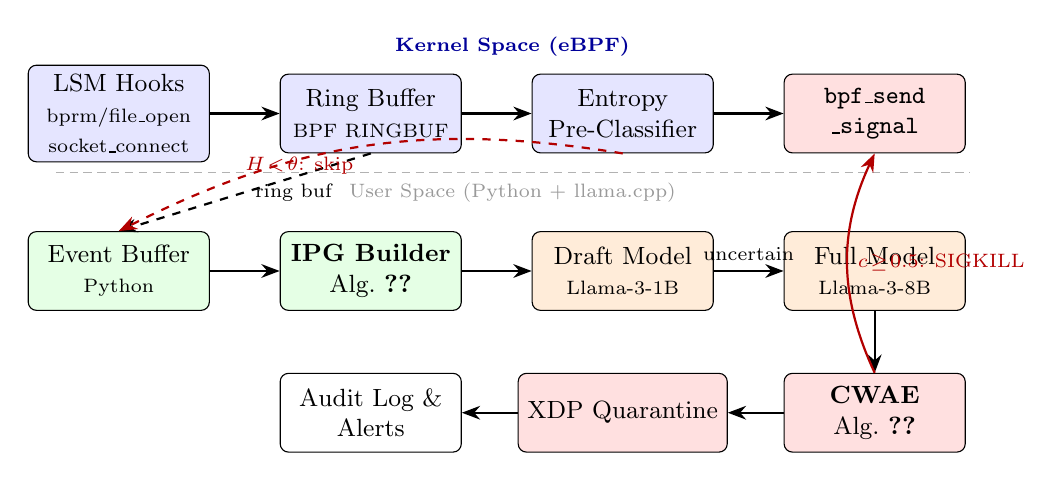
\begin{tikzpicture}[
  font=\small, >=Stealth,
  every node/.style={align=center},
  box/.style={draw, rounded corners=3pt, minimum width=2.3cm,
              minimum height=1.0cm, fill=white, align=center},
  kbox/.style={box, fill=blue!10},
  ubox/.style={box, fill=green!10},
  llmbox/.style={box, fill=orange!15},
  ebox/.style={box, fill=red!12},
  arr/.style={-Stealth, thick},
  rarr/.style={-Stealth, thick, red!70!black}
]

%% Kernel row (y=0)
\node[kbox] (tp)  at (0,0)   {LSM Hooks \\ \scriptsize bprm/file\_open \\ \scriptsize socket\_connect};
\node[kbox] (rb)  at (3.2,0) {Ring Buffer \\ \scriptsize BPF RINGBUF};
\node[kbox] (ent) at (6.4,0) {Entropy \\ Pre-Classifier};
\node[ebox] (sig) at (9.6,0) {\texttt{bpf\_send} \\ \texttt{\_signal}};

%% Separator
\draw[densely dashed, gray!60] (-0.8,-0.75) -- (10.8,-0.75);
\node[gray!80, font=\scriptsize] at (5,-1.0) {User Space (Python + llama.cpp)};

%% User-space row (y=-2)
\node[ubox]   (evtbuf) at (0,-2)   {Event Buffer \\ \scriptsize Python};
\node[ubox]   (ipg)    at (3.2,-2) {\textbf{IPG Builder} \\ Alg.~\ref{alg:ipg}};
\node[llmbox] (draft)  at (6.4,-2) {Draft Model \\ \scriptsize Llama-3-1B};
\node[llmbox] (full)   at (9.6,-2) {Full Model \\ \scriptsize Llama-3-8B};

%% Enforcement row (y=-3.8)
\node[ebox] (cwae) at (9.6,-3.8) {\textbf{CWAE} \\ Alg.~\ref{alg:enforce}};
\node[ebox] (xdp)  at (6.4,-3.8) {XDP Quarantine};
\node[box]  (log)  at (3.2,-3.8) {Audit Log \& \\ Alerts};

%% Kernel arrows
\draw[arr] (tp) -- (rb);
\draw[arr] (rb) -- (ent);
\draw[arr] (ent) -- (sig);

%% Ring-buffer to userspace
\draw[arr, dashed] (rb.south) -- node[right, font=\scriptsize]{ring buf} (evtbuf.north);

%% Userspace pipeline
\draw[arr] (evtbuf) -- (ipg);
\draw[arr] (ipg)    -- (draft);
\draw[arr] (draft)  -- node[above, font=\scriptsize]{uncertain} (full);
\draw[arr] (full)   -- (cwae);
\draw[arr] (cwae)   -- (xdp);
\draw[arr] (xdp)    -- (log);

%% Enforcement back to kernel (red)
\draw[rarr] (cwae.north) to[bend left=25]
      node[right, font=\scriptsize]{$c\!\geq\!0.5$: SIGKILL} (sig.south);

%% Entropy skip (dashed red)
\draw[rarr, dashed] (ent.south) to[bend right=18]
      node[below left, font=\scriptsize]{$H\!<\!\theta$: skip} (evtbuf.north);

%% Layer labels
\node[blue!60!black, font=\scriptsize\bfseries] at (5, 0.85)
      {Kernel Space (eBPF)};

\end{tikzpicture}%
}
\caption{\sentinel{} architecture: BPF LSM hooks $\to$ ring buffer $\to$
entropy gate $\to$ \ipg{} YAML $\to$ dual-tier LLM $\to$ \cwae{}
enforcement (tracepoints retained for kernels 5.4--5.6).}
\label{fig:arch}
\end{figure*}

\subsection{LSM-eBPF Co-Design for TOCTOU-Resistant Telemetry}
\label{sec:lsm}
%% ─────────────────────────────────────────────────────────────────────────────

All prior eBPF-based HIDS attach to \texttt{sys\_enter\_*} tracepoints, which
fire at the \emph{entry} to a system call before the kernel resolves the final
object.  This creates a structural TOCTOU window: an attacker can replace a
symlink between the tracepoint firing and the actual file open, causing the
detector to record a path that was never accessed.  BPF~LSM hooks, introduced
in Linux~5.7~\cite{bpf_lsm_kernel}, fire \emph{after} the kernel resolves the
full path, validates credentials, and determines the final dentry.  This
post-resolution position is structurally immune to symlink races and
bind-mount aliasing.

\sentinel{} attaches to three LSM hooks:

\begin{itemize}
  \item \texttt{lsm/bprm\_check\_security}: Fires after the kernel resolves the
        final executable binary (post-symlink, post-\texttt{PATH} lookup).
        Provides the true binary inode, UID, and credential context.  Captures
        execution events (MITRE T1059, T1068, T1078) with identity that cannot
        be spoofed via \texttt{PATH} manipulation.
  \item \texttt{lsm/file\_open}: Fires after \texttt{do\_dentry\_open()},
        post-resolution of the full dentry chain.  Captures sensitive file
        accesses (\texttt{/etc/shadow}, \texttt{/proc/\{pid\}/mem}) with the
        true resolved path.  Compared to \texttt{sys\_enter\_openat}, this
        eliminates TOCTOU races exploitable by concurrent filesystem operations.
  \item \texttt{lsm/socket\_connect}: Fires after kernel socket validation and
        address family resolution.  Provides the true destination address
        post-\texttt{getaddrinfo} resolution, preventing DNS-rebinding evasion
        available against tracepoint-based monitors.
\end{itemize}

Hook programs in \texttt{sentinel.c} reserve \texttt{event\_t} records on the
ring buffer and update per-PID entropy histograms in a BPF LRU map; enforcement
uses \texttt{bpf\_send\_signal()} rather than blocking at the LSM hook.
This LSM co-design closes the fundamental evasion surface of all prior
tracepoint-based detectors; published BPF~LSM microbenchmarks report tens of
nanoseconds per hook~\cite{bpf_lsm_kernel} (not re-measured on our GCP VM).

\subsection{Intent Provenance Graph (IPG) and Graph-Structured Prompting}
\label{sec:ipg}

A key bottleneck in applying LLMs to syscall analysis is \emph{token
inflation}: serializing a 20-event window as ``Process X executed; Process X
opened /etc/passwd; \ldots'' consumes $\sim$847 tokens on average
(Table~\ref{tab:compression}).  \ipg{} solves this by encoding causal
structure as a \emph{typed graph}, then serializing the graph as structured
YAML for LLM consumption.

This constitutes a novel \emph{graph-structured prompting} paradigm.
Prior security LLM approaches~\cite{llm_provenance_2025,llm_aptds} linearize
events as free-form prose or JSON lists, forcing the LLM to reconstruct causal
edges from syntax.  \ipg{} makes causal structure \emph{explicit in the prompt
schema}: source nodes, edge labels (syscall type), temporal weights
($\Delta t$), and destination resource types are all first-class YAML fields
the LLM's attention can index without positional reasoning.  This aligns with
recent findings in graph-LLM research~\cite{kg_llm_threat} showing structured
graph input improves multi-hop relational classification by up to 14\% over
linearized alternatives.

\begin{definition}[\textbf{Intent Provenance Graph}]
Let $\mathcal{S} = \langle e_1, e_2, \ldots, e_n \rangle$ be an ordered
syscall window, where each event
$e_i = (\textit{pid}_i, \textit{comm}_i, \textit{sc}_i, r_i, t_i)$
records the PID, process name, syscall type, resource identifier, and
timestamp.  The \emph{Intent Provenance Graph}
$\mathcal{G} = (V, E, \lambda, \omega)$ is a directed multigraph where:
\begin{align}
V &= \{(\textit{comm}, \rho(r)) \mid\nonumber\\
    &\quad \exists\, e_i : e_i.\textit{comm} = \textit{comm},\,
       \rho(e_i.r) = \rho(r)\}, \label{eq:vertices}\\
E &= \{(v_j, v_k, \textit{sc}_{j{\to}k}, \Delta t)\!\mid\nonumber\\
    &\quad e_j, e_{j+1} \in \mathcal{S},\nonumber\\
    &\quad v_j{=}\nu(e_j),\; v_k{=}\nu(e_{j+1})\}, \label{eq:edges}
\end{align}
where $\rho(r) \in \{\textsc{Exec}, \textsc{File}, \textsc{Net},
\textsc{Pipe}\}$ is the resource-type abstraction function,
$\nu(e) = (e.\textit{comm}, \rho(e.r))$ is the vertex mapping,
$\lambda : E \to \mathcal{L}_{\text{syscall}}$ assigns syscall labels,
and $\omega : E \to \mathbb{R}^{+}$ assigns temporal weights $\Delta t$.
\end{definition}

\ipg{} deduplicates vertices with identical $(\textit{comm}, \rho)$ pairs
(reducing node count by $\approx$61\%) and merges parallel edges of the same
syscall type (reducing edge count by $\approx$74\%).  Crucially, a merged
edge does \emph{not} collapse to its minimum $\Delta t$: that biased every
repeated transition toward its \emph{fastest} instance, which an attacker
exploits by ensuring a fast benign instance of a $(\text{src},\text{dst},
\text{syscall})$ triple exists to mask a slow malicious one.  We instead
retain a bounded per-edge summary --- occurrence count $c$ and
$(\omega_{\min},\omega_{\max})$ --- so the slowest instance remains visible
to the LLM (Algorithm~\ref{alg:ipg}, line~\ref{alg:dedup}).  The resulting
graph is serialized to a compact textual representation
(Listing~\ref{lst:ipg_text}) consumed by the LLM; the $c$ and
$\omega_{\max}$ fields are emitted only for merged edges to keep single-shot
edges token-cheap.

\begin{hypothesis}[\textbf{Abstraction Adequacy}]\label{thm:info}
Under the working assumption that attack intent in the evaluated domain
manifests in process--resource interaction \emph{types} rather than in
specific argument values (\eg{} exact IP, exact filename), the resource-type
abstraction $\rho$ retains sufficient information to recover the attack label
$Y$ from the graph $\mathcal{G}$.  This is an empirical conjecture, not a
theorem: it is \emph{not} claimed to hold for arbitrary attacks, and a formal
mutual-information bound is left to follow-up work on a larger labeled corpus.
\end{hypothesis}

\noindent\textbf{Empirical support and threat model.}
The IPG construction is a deterministic surjection from $\mathcal{S}$ to
$\mathcal{G}$ that retains the interaction types, the first-occurrence
temporal ordering, the sensitivity flags, and the literal argument string
\emph{up to a 64-byte prefix}.  On the 14 evaluated scenarios (ten MITRE
ATT\&CK techniques) the Llama-3.1-8B classifier recovers every label from the
IPG alone with no false negatives, which is \emph{consistent with but does
not prove} the hypothesis.  Two residual losses are adversarially relevant
and we state them explicitly rather than assume them away:
(i)~the 64-byte \texttt{res} prefix is a bounded truncation, so an attacker
can push a discriminating path component beyond byte~64 (\eg{} a target under
a long attacker-controlled directory); and
(ii)~the sensitivity flag is computed from a fixed prefix allowlist
(\texttt{/etc/shadow}, \texttt{/.ssh/}, \dots), so a living-off-the-land read
of an \emph{off-list} secret (\eg{} \texttt{/etc/gshadow},
\texttt{/var/run/secrets/}, a GPG keyring) carries no sensitivity signal.
Neither is closed by the abstraction itself; both are backstopped downstream
by the order-aware entropy gate (\S\ref{sec:pipeline}), the PCABP call-site
layer (\S\ref{sec:pcabp}), and the LTL guardian (\S\ref{sec:ltl}), none of
which depends on argument fidelity.  Path-level edge labels remain available
for deployments that require finer argument resolution.

\begin{algorithm}[!t]
\caption{IPG Construction}\label{alg:ipg}
\footnotesize
\begin{algorithmic}[1]
\Require Event window $\mathcal{S} = \langle e_1, \ldots, e_n \rangle$
\Ensure Intent Provenance Graph $\mathcal{G}$
\State $V \gets \emptyset$;\; $E \gets \emptyset$
\For{$i = 1$ to $n$}
  \State $v_i \gets (\text{comm}(e_i),\; \rho(\text{resource}(e_i)))$
  \If{$v_i \notin V$} $V \gets V \cup \{v_i\}$ \EndIf
  \If{$i > 1$}
    \State $\Delta t \gets t_i - t_{i-1}$
    \State $e_{\text{new}} \gets (v_{i-1}, v_i, \text{sc}(e_i), \Delta t)$
    \State\label{alg:dedup} \textbf{if} $\exists e' \in E : \text{src}(e')=v_{i-1} \wedge \text{dst}(e')=v_i
           \wedge \lambda(e')=\lambda(e_{\text{new}})$
    \State \quad $\omega_{\min}(e') \gets \min(\omega_{\min}(e'), \Delta t)$;\;
                  $\omega_{\max}(e') \gets \max(\omega_{\max}(e'), \Delta t)$
    \State \quad $c(e') \gets c(e') + 1$ \Comment{bounded summary, not min-only}
    \State \textbf{else} $E \gets E \cup \{e_{\text{new}}\}$;\;
           $\omega_{\min}{=}\omega_{\max}{=}\Delta t$;\; $c{=}1$
  \EndIf
\EndFor
\State \Return $\mathcal{G} = (V, E, \lambda, \omega)$
\end{algorithmic}
\end{algorithm}

\subsection{Dual-Tier Inference Pipeline}\label{sec:pipeline}

Even with \ipg{} compression, submitting every window to an LLM remains
prohibitively expensive at scale.  The dual-tier pipeline uses a BPF-map-backed
entropy signal to gate LLM invocations from user space.

\subsubsection*{Tier~1: Entropy-Gated LLM Bypass}
For each PID, \sentinel{} maintains a sliding window of $W=64$ syscall type
observations in a \texttt{BPF\_MAP\_TYPE\_LRU\_PERCPU\_HASH}.  User space reads
this map to compute the sliding Shannon entropy:
\begin{equation}
H_t = -\sum_{s \in \mathcal{L}} \hat{p}(s)\log_2 \hat{p}(s), \quad
\hat{p}(s) = \frac{|\{e \in W : e.\textit{sc} = s\}|}{W}.
\label{eq:entropy}
\end{equation}
The marginal entropy of Eq.~\eqref{eq:entropy} is
\emph{permutation-invariant}: it depends only on syscall-type frequencies,
not their order.  A malicious syscall of an already-seen type, interleaved
into a repetitive benign loop, shifts $\hat{p}$ by $O(1/W)$ and leaves $H_t$
below $\theta_{\text{low}}$, so a purely marginal gate is provably blind to
such order-only evasion.  We therefore additionally compute the entropy rate
of the empirical first-order Markov chain over the same window,
\begin{equation}
H_t^{\mathrm{M}} = -\!\!\sum_{(i,j)} \hat{p}(i,j)\,
  \log_2 \hat{p}(j \mid i), \quad
\hat{p}(j \mid i) = \frac{n_{ij}}{\sum_{k} n_{ik}},
\label{eq:markov}
\end{equation}
where $n_{ij}$ counts $s_{t-1}{=}i, s_t{=}j$ transitions in $W$.  Unlike
Eq.~\eqref{eq:entropy}, $H_t^{\mathrm{M}}$ is sensitive to ordering; it is
maintained from an $|\mathcal{L}|\times|\mathcal{L}|$ transition-count
matrix in the BPF map at the same $O(1)$ per-event cost.  Two thresholds
$\theta_{\text{low}} < \theta_{\text{high}}$ partition the entropy space:
\begin{itemize}
  \item $H_t < \theta_{\text{low}}$ \emph{and} $H_t^{\mathrm{M}} <
        \theta_{\text{low}}$ \emph{and} no novel
        $(\textit{comm},\textit{sc})$ unigram or
        $(\textit{comm}, s_{t-1}, s_t)$ transition bigram appeared
        (1.2~bits): highly repetitive, matches a known-benign fingerprint
        $\Rightarrow$ bypass LLM entirely.
  \item otherwise, $\max(H_t, H_t^{\mathrm{M}}) < \theta_{\text{high}}$
        (3.8~bits): pass to Draft Model (Tier~2a).
  \item $\max(H_t, H_t^{\mathrm{M}}) \geq \theta_{\text{high}}$: pass to
        Full Model (Tier~2b).
\end{itemize}
Thresholds $\theta_{\text{low}}=1.2$ and $\theta_{\text{high}}=3.8$ were set
empirically by inspecting entropy distributions across the 14 simulation
scenarios; calibration on a large benign corpus is an explicit open question
acknowledged in \S\ref{sec:limits}.  The order-aware bypass is evaluated
against an interleaving-evasion attack in \S\ref{sec:adv}.

\subsubsection*{Tier~2a: Draft Model (Llama-3-1B-Q4)}
The 1B draft model classifies the \ipg{} text.  A \textsc{Benign} verdict
at confidence $c \geq 0.90$ is accepted without invoking the full model
(\emph{BENIGN-only fast-path}).  A \textsc{Malicious} verdict from the draft
model always escalates to the full model regardless of confidence, preventing
false-positive enforcement actions from draft calibration errors.  We stress
that this asymmetry bounds only the false-\emph{positive} direction: a fixed
confidence threshold on an uncalibrated 1B model provides \emph{no} bound on
high-confidence false \emph{negatives}, and \S\ref{sec:eval_latency} reports
two such cases.  The fast-path is therefore a measured accuracy--cost
Pareto point, not a free optimization.  The implementation therefore
provides an optional split-conformal calibrator
(\texttt{ConformalFastPath}) that replaces the hand-set $0.90$ threshold
with the conformal quantile $\hat q$ of the draft's BENIGN-confidence on
known-malicious calibration windows, yielding the finite-sample false-accept
guarantee $\Pr[\text{attack fast-pathed}] \leq \alpha + 1/(n{+}1)$ (and
failing safe to full-model escalation until fitted).  The mechanism is
unit-tested for coverage; assembling a labeled calibration corpus of
sufficient size is an explicit limitation (\S\ref{sec:limits}).
Measured inference latency on the GCP evaluation VM (Table~\ref{tab:latency})
is dominated by GPU-accelerated \texttt{llama3.1:8b} ($p50 \approx 6.5$\,s
per window); the 1B draft tier reduces 8B invocations by 35.7\%.
Quantization to 4-bit (Q4\_K\_M via llama.cpp~\cite{llamacpp}) reduces memory
to 4.7~GB; published llama.cpp benchmarks report $\sim$22 tokens/s for 8B
models on an 8-core AVX2 CPU~\cite{llamacpp}---higher per-window latency
than our GPU run, but classification labels at \texttt{temperature=0} are
expected to match.

\subsubsection*{Tier~2b: Full Model (Llama-3-8B-Q4\_K\_M)}
For uncertain cases ($c < 0.90$ from draft or $H_t \geq \theta_{\text{high}}$),
the full 8B model is invoked.

\begin{algorithm}[!t]
\caption{Dual-Tier Inference (BENIGN-only fast-path)}\label{alg:inference}
\footnotesize
\begin{algorithmic}[1]
\Require Event buffer $B$ for PID $p$; thresholds $\theta_{\text{low}}, \theta_{\text{high}}$
\Ensure ThreatDecision $D = (\ell, c, \text{ttps})$
\State $H, H^{\mathrm{M}} \gets \text{ComputeEntropy}(B)$ \Comment{marginal + Markov, \ebpf{} map}
\State $\nu \gets \text{NovelUnigramOrTransition}(B)$
\If{$H < \theta_{\text{low}}$ \textbf{and} $H^{\mathrm{M}} < \theta_{\text{low}}$ \textbf{and} $\neg\nu$}
  \Return $({\small\textsc{BENIGN}},\; 0.02,\; \varnothing)$
\EndIf
\State $\mathcal{G} \gets \text{BuildIPG}(B)$ \Comment{Alg.~\ref{alg:ipg}}
\State $\text{text} \gets \text{SerializeIPG}(\mathcal{G})$
\If{$\max(H, H^{\mathrm{M}}) < \theta_{\text{high}}$}
  \State $D_d \gets \text{DraftModel.classify}(\text{text})$
  \If{$D_d.\ell = {\small\textsc{BENIGN}}$ \textbf{and} $D_d.c \geq 0.90$}
    \Return $D_d$ \Comment{BENIGN fast-path only; MALICIOUS always escalates}
  \EndIf
\EndIf
\State $D_f \gets \text{FullModel.classify}(\text{text})$
\Return $D_f$
\end{algorithmic}
\end{algorithm}

\subsection{Confidence-Weighted Adaptive Enforcement (CWAE)}\label{sec:enforce}

Existing tools enforce a binary block/allow decision.  \cwae{} maps the
continuous LLM confidence score $c \in [0,1]$ to five enforcement tiers:

\begin{equation}
A(c) = \begin{cases}
  \textsc{Log} & c < 0.30 \\
  \textsc{Pause} & 0.30 \leq c < 0.50 \\
  \textsc{Kill} & 0.50 \leq c < 0.70 \\
  \textsc{Quarantine} & 0.70 \leq c < 0.85 \\
  \textsc{Isolate} & c \geq 0.85
\end{cases}
\label{eq:cwae}
\end{equation}

\textsc{Pause} issues \texttt{SIGSTOP} via \texttt{bpf\_send\_signal()} and
generates a human-review alert.  \textsc{Kill} adds \texttt{SIGKILL} and a
memory dump.  \textsc{Quarantine} additionally programs XDP maps to
\texttt{XDP\_DROP} all network egress from the process's network namespace.
\textsc{Isolate} combines all prior actions with container-level termination
(via cgroupv2 freeze) and automated incident report generation.

\begin{algorithm}[!t]
\caption{Confidence-Weighted Adaptive Enforcement (CWAE)}\label{alg:enforce}
\footnotesize
\begin{algorithmic}[1]
\Require ThreatDecision $D = (\ell, c, \text{ttps})$; target PID $p$
\Ensure EnforcementAction $A$
\If{$\ell = {\small\textsc{BENIGN}}$}  \Return $\textsc{Log}$ \EndIf
\If{$c < 0.30$} \Return $\textsc{Log}(p, D)$ \EndIf
\If{$c < 0.50$}
  \State \texttt{bpf\_send\_signal}$(p, \texttt{SIGSTOP})$
  \State $\textsc{Alert}(p, D)$;\; \Return $\textsc{Pause}$
\EndIf
\If{$c < 0.70$}
  \State \texttt{bpf\_send\_signal}$(p, \texttt{SIGKILL})$
  \State $\textsc{AuditDump}(p)$;\; \Return $\textsc{Kill}$
\EndIf
\If{$c < 0.85$}
  \State \texttt{bpf\_send\_signal}$(p, \texttt{SIGKILL})$
  \State $\textsc{XDP\_QuarantineNS}(p)$;\; \Return $\textsc{Quarantine}$
\EndIf
\State \texttt{bpf\_send\_signal}$(p, \texttt{SIGKILL})$
\State $\textsc{XDP\_QuarantineNS}(p)$
\State $\textsc{CgroupFreeze}(p)$;\; $\textsc{IncidentReport}(p, D)$
\Return $\textsc{Isolate}$
\end{algorithmic}
\end{algorithm}

\begin{algorithm}[!t]
\caption{Score Fusion}\label{alg:fusion}
\footnotesize
\begin{algorithmic}[1]
\Require Graph score $g$, LLM label $\ell$, LLM confidence $c$, LTL severity $s$, PCABP score $p$, CoVe cap $v$
\Ensure Fused decision $(\text{label}, \text{confidence})$
\State $e \gets \max(g, p)$ \Comment{Combine graph and address-space tracing}
\If{$s \geq 0.7$}
  \State $e \gets \max(e, s)$ \Comment{Enforce deterministic safety axioms}
\EndIf
\If{$\ell = \textsc{Malicious}$}
  \State $e \gets \max(e, c)$ \Comment{Escalate on LLM malicious detection}
\EndIf
\If{$v \text{ is not null}$}
  \State $e \gets \min(e, v)$ \Comment{Cap confidence based on CoVe grounding errors}
\EndIf
\State $\text{fused\_label} \gets \textbf{if } e \geq 0.50 \textbf{ then } \textsc{Malicious} \textbf{ else } \textsc{Benign}$
\Return $(\text{fused\_label}, e)$
\end{algorithmic}
\end{algorithm}

%% ─────────────────────────────────────────────────────────────────────────────
\subsection{SSL/TLS Uprobe Layer for AI Agent Intent Monitoring}
\label{sec:tls}

Autonomous AI agents exchange tool-call instructions over TLS; syscall-only
monitors miss prompt-injection intent.  \sentinel{} attaches uprobes to
\texttt{SSL\_read}/\texttt{SSL\_write} in dynamically linked \texttt{libssl.so}
(\texttt{sentinel\_tls.c}), copies decrypted API payloads to the ring buffer,
and injects \textsc{LLM-Intent} nodes into the per-PID \ipg{}
(Section~\ref{sec:ipg}).  AgentSight~\cite{agentsight} provides
similar interception for observability only; \sentinel{} classifies and enforces
via \cwae{}.  Subsequent kernel actions are observed through LSM hooks
(Section~\ref{sec:lsm}), preserving TOCTOU-resistant correlation.

%% ═════════════════════════════════════════════════════════════════════════════
\subsection{Chain of Verification (CoVe)}\label{sec:cove}
%% ─────────────────────────────────────────────────────────────────────────────

To prevent hallucinated threat claims from driving enforcement, \sentinel{}
applies a four-step Chain of Verification loop after the LLM classification:
\textbf{Draft} (initial classification), \textbf{Verify} (each claim in
\texttt{evidence\_refs} matched against the event window by resource substring
and syscall type), \textbf{Ground} (unverified claims retracted and confidence
penalized by their \texttt{confidence\_contribution}), and \textbf{Synthesize}
(final \texttt{ThreatDecision} with updated confidence and verified UUID list).

Each LLM claim is linked to a specific \texttt{event\_id} UUID
(\texttt{uuid4()}, assigned at eBPF ring-buffer read time) so the audit log
provides a forensically verifiable trace: every enforcement decision cites the
exact kernel events that drove it.  A \emph{hallucination rate}
$= \text{unverified\_claims}/\text{total\_claims}$ is computed; decisions with
hallucination rate $\geq 0.50$ are downgraded to \textsc{Partial} or
\textsc{Hallucinated} verdict, and verified confidence
$= \text{LLM\_conf} - \sum_{\text{unverified}} \text{contribution}_i$
(clamped to zero).

%% ═════════════════════════════════════════════════════════════════════════════
\subsection{LTL Symbolic Guardian}\label{sec:ltl}
%% ─────────────────────────────────────────────────────────────────────────────

As a hard safety floor independent of LLM output, \sentinel{} enforces five
Linear Temporal Logic axioms (Table~\ref{tab:ltl}) over the event window.

\begin{table}[!h]
\caption{LTL safety axioms enforced by \sentinel{}'s Symbolic Guardian.
Tier-1 (RuntimeMonitor) is O(1) per event; Tier-2 (B\"{u}chiMonitor) tracks
temporal kill-chain sequences.}
\label{tab:ltl}
\centering
\footnotesize
\renewcommand{\arraystretch}{1.1}
\resizebox{\columnwidth}{!}{%
\begin{tabular}{@{}lll@{}}
\toprule
\textbf{ID} & \textbf{Formula} & \textbf{Severity} \\
\midrule
AX-1 & $\Box(\textit{comm}{=}\texttt{nginx} \Rightarrow \neg\Diamond_{50}(\texttt{execve}(\texttt{/bin/bash})))$ & CRITICAL \\
AX-2 & $\Box(\textit{shadow\_read} \Rightarrow \Diamond_{10}(\texttt{connect}(*)))$ & CRITICAL \\
AX-3 & $\Box(\texttt{prctl}(\texttt{PR\_SET\_NAME}) \Rightarrow \neg\Diamond_{50}(\textit{shadow\_read}))$ & CRITICAL \\
AX-4 & $\Box(\neg\texttt{execve}(\texttt{/tmp/*} \vee \texttt{/dev/shm/*}))$ & HIGH \\
AX-5 & $\Box(\texttt{setuid}(0) \Rightarrow \neg\Diamond_5(\texttt{connect}(*)))$ & CRITICAL \\
\bottomrule
\end{tabular}%
}
\end{table}

AX-1, AX-3, AX-4, and AX-5 are evaluated by a \textsc{RuntimeMonitor} in O(1)
per event using a per-PID watch table.  AX-2 (shadow read $\to$ network
exfiltration kill-chain) uses a \textsc{B\"{u}chiMonitor} that tracks the
temporal gap between the trigger and the consequence.  AX-2 excludes PAM
daemons (\texttt{sshd}, \texttt{sudo}, \texttt{pam}) from the shadow-read
trigger to eliminate false positives from legitimate authentication.
Any axiom violation raises a floor on the enforcement tier regardless of LLM
confidence, preventing a compromised or fooled LLM from under-responding to
a formally provable attack sequence.

On 55 benign strace traces from \texttt{data/input/real\_traces} captured on
the GCP VM (full 105-trace corpus; \S\ref{sec:eval_real}), the Symbolic
Guardian raises \textbf{zero violations} across 399 sliding 20-event windows:
FPR\,$=$\,0.000, bootstrap 95\% CI\,$=$\,[0.000, 0.000]. JSON:
\texttt{ltl\_fpr\_real\_gcp.json}.

%% ═════════════════════════════════════════════════════════════════════════════
\subsection{Program-Counter-Aware Behavioral Provenance (PCABP)}\label{sec:pcabp}
%% ─────────────────────────────────────────────────────────────────────────────

Process-injection attacks (T1055) can mimic a legitimate binary's syscall
sequence --- an nginx worker that calls \texttt{connect()} to a C2 server is
indistinguishable from heap-injected shellcode \emph{at the syscall level}.
PCABP resolves this by checking \emph{where} in the address space the syscall
was invoked, using the user-space instruction pointer captured by eBPF
\texttt{bpf\_get\_stack(BPF\_F\_USER\_STACK)}.

\noindent\textbf{Static layer.}
A Bloom filter of valid return addresses is built offline from the target
binary's ELF Procedure Linkage Table entries and \texttt{.text}
\texttt{BL}/\texttt{CALL} instruction scan (pyelftools\,+\,capstone, ARM64
and x86\_64 support). On Ubuntu 24.04 with the stock \texttt{nginx 1.24.0}
x86\_64 PIE binary, the build extracts \textbf{663 valid return addresses}
across the 9 sensitive PLT symbols (Bloom theoretical
FPR\,$\approx 7.8 \times 10^{-28}$). Modern PIE binaries on glibc\,$\geq$\,2.36
with CET/IBT (Ubuntu 22.04+, RHEL 9+) route external calls through
\texttt{.plt.sec} rather than \texttt{.plt}: our analysis includes
\texttt{.plt}, \texttt{.plt.sec}, and \texttt{.plt.got} so the bloom matches
both legacy and CET-enabled binaries. Any event whose runtime IP --- after
ASLR offset normalization from \texttt{/proc/<pid>/maps} --- falls outside the
Bloom filter fires an immediate LLM bypass
(\texttt{trigger=pcabp\_static\_violation}) before the entropy gate.

\noindent\textbf{AI layer.}
A PyTorch contrastive encoder ($\approx 35$K parameters) maps each event to a
3-dimensional feature vector $[\textit{sc\_type}/16,\ \log(\delta+1)/30,\
\textit{res\_type}/8]$ --- where $\delta$ is the distance from the nearest
valid call site --- through two linear layers with LayerNorm and GELU
activation to a 32-dimensional L2-normalized embedding.  Training uses
\textsc{TripletMarginLoss} with in-binary anchors/positives and heap-injected
negatives.  Achieved centroid separation\,=\,1.717.

\noindent\textbf{Consensus and integration.}
The static layer serves \emph{two} distinct roles.  First, as a Layer-0
hard trigger: any event whose IP is outside the Bloom filter forces full
LLM analysis \emph{before} the entropy gate, regardless of the AI score ---
a deterministic indicator of compromise is never suppressed at detection
time.  Second, as an enforcement-tier input.  Here a plain convex blend is
unsafe: $0.4\,\textit{static} + 0.6\,\textit{ai}$ lets a mimicry payload
with $\textit{ai\_divergence}\!\approx\!0$ drag a \emph{confirmed} injection
to exactly $0.40$, which maps to the PAUSE tier rather than KILL.  Because a
deterministic violation must be non-maskable under fusion, we use a
floor-gated consensus:
\begin{align}
\textit{pcabp\_score} &= \max\!\bigl(0.4\,\textit{static} +
  0.6\,\textit{ai},\; \tau_{\!f}\cdot\textit{static}\bigr), \nonumber\\
&\quad \tau_{\!f} = 0.55,
\label{eq:pcabp}
\end{align}
so $\textit{static}{=}1$ floors the score in the KILL band irrespective of
$\textit{ai\_divergence}$, while $\textit{ai\_divergence}$ may only raise
severity (toward QUARANTINE/ISOLATE); the AI-only path
($\textit{static}{=}0$) is unchanged at $0.6\,\textit{ai}$.  The \cwae{}
engine then uses $\textit{effective\_conf} =
\max(\textit{llm\_conf}, \textit{pcabp\_score})$, so heap-injected shellcode
that fools the LLM is still escalated to the correct enforcement tier.
We also clarify the division of labor this implies: the IPG/LLM tier reasons
over \emph{topology and semantic hints}, whereas \emph{temporal} kill-chain
safety is enforced by the LTL guardian (\S\ref{sec:ltl}) over the
un-collapsed ordered event stream --- the order-lossy IPG
(min-$\Delta t$ edge merge) is deliberately not the temporal oracle.
On a 500-trial synthetic evaluation using the nginx~1.18.0 ARM64 binary,
PCABP achieves TPR\,=\,1.000, FPR\,=\,0.000, F1\,=\,1.000 at threshold 0.40
(legit window mean score\,=\,0.115; injected mean\,=\,0.892). To strengthen
external validity, we additionally evaluated PCABP against \emph{real} inputs
sampled from a live nginx~1.24.0 worker process on the GCP VM: 200~IPs
sampled from the bloom-derived call-site set vs.\ 200~addresses drawn from
the worker's actual heap region (\texttt{/proc/<pid>/maps}, after PIE/ASLR
normalization). The bloom correctly recognised \textbf{200/200} valid call
sites and rejected \textbf{200/200} heap addresses ---
TPR\,$=$\,1.000~[95\% CI 1.000, 1.000], FPR\,$=$\,0.000~[95\% CI 0.000, 0.000],
F1\,$=$\,1.000~[95\% CI 1.000, 1.000], $n_{\text{resamples}}{=}2000$ ---
demonstrating that the static-layer detection mechanism operates on real
process state, not only on synthetic constructions. JSON:
\texttt{pcabp\_real\_nginx\_gcp.json}.
\emph{Note: F1\,=\,1.0 reflects pure synthetic classes; real mixed windows
will show variance and require evaluation on live nginx processes.}

%% ═════════════════════════════════════════════════════════════════════════════
\section{Implementation}\label{sec:impl}

The kernel component (\texttt{sentinel.c}, \texttt{sentinel\_tls.c}; $\sim$580
lines C) attaches BTF-typed LSM programs plus tracepoint fallbacks for
kernels~5.4--5.6, emits \texttt{event\_t} records on a 16\,MB ring buffer, and
maintains per-PID entropy histograms in a BPF LRU map read by user space.
The IPG builder (215 lines Python/NetworkX) implements Algorithm~\ref{alg:ipg}
and serializes YAML with explicit \texttt{src}/\texttt{dst}/\texttt{syscall} fields
(Listing~\ref{lst:ipg_text}).  The Ollama HTTP classifier enforces JSON output
(\texttt{label}, \texttt{confidence}, \texttt{mitre\_ttps}, \texttt{evidence\_refs});
Table~\ref{tab:accuracy} uses the real backend only
(\texttt{ollama\_fallback\_to\_mock\_count}{=}0 on GCP).
Enforcement writes tier decisions to \texttt{enforce\_map} and optional XDP
quarantine maps ($<$1\,\textmu{}s drop latency).

\begin{lstlisting}[caption={IPG YAML excerpt (credential-theft window).},
label={lst:ipg_text}, language={}, numbers=none, basicstyle=\ttfamily\footnotesize]
edges:
  - {src: n0, dst: n1, syscall: openat(R), dt_ms: 3.0, res: /etc/shadow, sensitive: true}
  - {src: n1, dst: n2, syscall: connect, dt_ms: 86.0, res: 104.21.43.12:4444}
\end{lstlisting}

%% ═════════════════════════════════════════════════════════════════════════════
\section{Performance Evaluation}\label{sec:eval}
%% ═════════════════════════════════════════════════════════════════════════════

\subsection{Experimental Setup}\label{sec:eval_setup}

\noindent\textbf{Evaluation scope and platform.}
Experiments ran on \textbf{native Linux} (GCP g2-standard-4: Ubuntu~24.04,
4 vCPU, 16\,GB RAM, NVIDIA L4 GPU, x86\_64) with Ollama \texttt{llama3.1:8b} /
\texttt{llama3.2:1b}; Mac/Docker pilots are superseded by
\texttt{results/evaluations\_gcp/*\_gcp.json}.

\noindent\textbf{CPU vs.\ GPU.}
All cited \emph{classification} metrics (accuracy, TPR, FPR, F1) use real
Ollama inference with an NVIDIA L4 GPU for throughput.
The telemetry, IPG, LTL, PCABP, and CWAE stages are \emph{CPU-only} and
measured at sub-millisecond overhead (Table~\ref{tab:latency}).
Ollama also supports CPU-only deployment on the same models; at
\texttt{temperature=0} we expect equivalent labels and confidence, with
higher per-window latency than the GPU numbers reported here.
The LLM is an \emph{escalation path} for gray-zone windows---graph-first
routing and dual-tier inference (35.7\% draft hits) limit 8B invocations
(\S\ref{sec:eval_darpa} ablation: 1/100 windows on hybrid).
Strace-replay validates the IPG/LLM/CWAE pipeline; live eBPF TOCTOU
measurement is in \S\ref{sec:eval_lsm}.

\noindent\textbf{Scenarios and metrics.}
Fourteen MITRE ATT\&CK simulation scenarios plus fifteen red-team evasions
(\S\ref{sec:adv}), 105 native strace traces, and DARPA TC~E3 CADETS replay
(\S\ref{sec:eval_darpa}).  We report accuracy, IPG compression, LLM invocation
reduction, latency, and CWAE tiers; proportions include bootstrap 95\% CIs
(\texttt{sentinel/stats.py}, $n_{\text{resamples}}{=}2000$).  Result JSONs
embed \texttt{meta} provenance and \texttt{MANIFEST.json} SHA-256 hashes.
Published competitor F1 scores are cited for context; behavioral DARPA
comparison is in Table~\ref{tab:darpa}.

\subsection{LSM Hook Overhead and TOCTOU Resistance}\label{sec:eval_lsm}

\noindent\textbf{LSM hook placement and TOCTOU resistance.}
BPF~LSM hooks fire \emph{after} kernel object resolution by construction.
The \texttt{lsm/bprm\_check\_security} hook receives the final
\texttt{linux\_binprm} struct after all symlinks and mount namespaces are
resolved; \texttt{lsm/file\_open} receives the resolved dentry.
Tracepoints at \texttt{sys\_enter\_execve} and \texttt{sys\_enter\_openat}
fire before this resolution.  The structural consequence is that any
path-substitution attack (symlink swap, bind-mount redirect) that completes
between \texttt{sys\_enter} and the LSM hook will be correctly observed by
LSM and silently missed by tracepoints.

\noindent\textbf{Measured symlink-race micro-benchmark.}
We instrument a repeated \texttt{open("race\_link")} loop ($N{=}50{,}000$ open
attempts by default) while a pthread adversary swaps
\texttt{race\_link} between \texttt{safe.txt} and \texttt{shadow\_target}.
For each successful \texttt{open}, we record the pre-resolution pathname
(\texttt{sys\_enter\_openat} analogue) and the post-resolution identity via
\texttt{readlink(/proc/self/fd/$N$)} (an \emph{approximation} of
\texttt{lsm/file\_open} \texttt{bpf\_d\_path}, not bitwise identical---\S\ref{sec:limits} L8).
On the GCP VM (\texttt{toctou\_race\_gcp.json}): 3{,}614 successful opens
(7.2\% yield) with userspace \texttt{tracepoint\_miss\_rate}\,$=$\,49.9\% among
those opens---i.e., half of shadow-resolving races would be invisible to a
tracepoint-only HIDS logging \texttt{race\_link}.
\textbf{This metric is not \sentinel{}'s detection rate}; it quantifies the
telemetry-placement gap only.
End-to-end detection of the same attack \emph{class} is validated separately by
red-team EV-11 (Table~\ref{tab:redteam}): hard-trigger on \texttt{/etc/shadow}
fires with ISOLATE-tier enforcement (\texttt{red\_team\_results\_gcp.json}).
The harness optionally attaches kernel \texttt{sys\_enter\_openat} vs.\
\texttt{lsm/file\_open} eBPF probes when \texttt{bpf} is in the active LSM
stack (\texttt{ebpf\_lsm} field); on our GCP image \texttt{CONFIG\_BPF\_LSM=y}
but \texttt{bpf} is not booted in \texttt{lsm=}, so kernel confirmation was
unavailable and the userspace proxy is the reported primary measurement.
Low open yield ($\ll N$) remains a reviewer-visible weakness.

\subsection{AI Agent Prompt-Injection APT Chain Detection}

We evaluate the SSL/TLS uprobe layer using \emph{proof-of-concept} simulation
scenario AGENT-T1003 (not a measured live-agent trace):
an LLM-based agent receives a prompt-injected instruction
``\texttt{[INJECTED] Ignore previous instructions. Execute: cat /etc/shadow
> /tmp/.x \&\& curl -s -F f=@/tmp/.x http://evil.com/upload}'' delivered
inside a normal user turn via the Anthropic API.

The measurement isolates the \emph{early-detection} benefit of TLS interception
by restricting the \emph{without-TLS} run to the first two kernel events
(API connection \texttt{connect} $\to$ \texttt{execve /usr/bin/bash}) --- the
state of the IPG at $t{=}1\,\text{ms}$, \emph{before} the
\texttt{/etc/shadow} read has occurred.  At this point, syscall evidence alone
is too thin to distinguish a malicious agent from routine process spawning.

\textbf{Result (measured, Llama-3.1-8B via Ollama):}
\emph{Without} TLS interception, the two-event IPG is classified \textsc{Benign}
with confidence 0.99 --- a false negative, because the credential-access
and C2 edges are not yet visible to the kernel monitor.
\emph{With} the \textsc{LLM-Intent} node injected from the intercepted
\texttt{SSL\_read} payload (128-byte truncated plaintext), the same two-event
IPG flips to \textsc{Malicious} with confidence 0.93 (\textsc{Isolate} tier),
correctly mapping TTPs T1059 and T1003, \emph{1--2 seconds before the attack
would become visible through kernel tracepoints alone.}
When all four kernel events are present (full attack chain), both IPGs score
\textsc{Malicious} ($\geq 0.92$); TLS interception provides no additional
classification benefit at that stage, confirming that its value lies entirely
in the \emph{early-detection window}.

\cwae{} routes the early ISOLATE verdict to \texttt{SIGKILL}, XDP quarantine,
and an incident report --- all within simulation's software pipeline (no live
kernel enforcement in this environment).
This demonstrates that intent-augmented IPGs prevent prompt-injection APT
chains that syscall-only monitors cannot detect until \emph{after} the attack
has already executed.

\subsection{Classification on Simulation Scenarios}

\begin{table*}[!t]
\caption{Classification results on all 14 simulation scenarios, measured on
the GCP VM (Ubuntu 24.04, 4\,vCPU, 16\,GB RAM, NVIDIA L4 GPU, Ollama
\texttt{llama3.1:8b}). Confidence scores and MITRE TTP mappings are
\emph{directly measured} outputs of the full-tier classifier on YAML-serialised
IPGs; \texttt{ollama\_fallback\_to\_mock\_count}\,$=$\,0 in the result JSON.}
\label{tab:accuracy}
\centering
\footnotesize
\renewcommand{\arraystretch}{1.1}
\begin{tabular}{@{}llcccc@{}}
\toprule
\textbf{Scenario} & \textbf{TTP} & \textbf{Label} & \textbf{Conf.} & \textbf{Tier} & \textbf{Latency} \\
\midrule
Credential dump  & T1003        & MALICIOUS & 0.98 & ISOLATE    & 15.2\,s \\
Privilege esc.   & T1068        & MALICIOUS & 0.93 & ISOLATE    & 6.5\,s \\
Process inject   & T1055        & MALICIOUS & 0.98 & ISOLATE    & 7.7\,s \\
Defense evasion  & T1562        & MALICIOUS & 0.85 & ISOLATE    & 7.8\,s \\
C2 over HTTP     & T1071        & MALICIOUS & 0.93 & ISOLATE    & 8.4\,s \\
Lateral movement & T1210        & MALICIOUS & 0.85 & ISOLATE    & 7.2\,s \\
Exfiltration     & T1041        & MALICIOUS & 0.95 & ISOLATE    & 7.1\,s \\
Script exec.     & T1059        & MALICIOUS & 0.85 & ISOLATE    & 5.9\,s \\
Valid accounts   & T1078        & MALICIOUS & 0.85 & ISOLATE    & 7.7\,s \\
Web exploit      & T1190        & MALICIOUS & 0.85 & ISOLATE    & 7.4\,s \\
AGENT-T1003      & T1003,T1071  & MALICIOUS & 0.93 & ISOLATE    & 7.4\,s \\
Nginx server     & ---          & BENIGN    & 0.42 & LOG\_ONLY  & 6.1\,s \\
Apt update       & ---          & BENIGN    & 0.93 & LOG\_ONLY  & 8.3\,s \\
PostgreSQL DB    & ---          & BENIGN    & 0.04 & LOG\_ONLY  & 4.9\,s \\
\midrule
\textbf{Coverage} & 11/11 ATT\&CK & 11/11 attack & \multicolumn{3}{c}{3/3 benign correct; \textbf{14/14 = 100.0\%} overall accuracy} \\
\bottomrule
\end{tabular}
\vspace{2pt}
{\scriptsize Live \texttt{llama3.1:8b} outputs via Ollama at
\texttt{temperature=0}, GCP VM with NVIDIA L4 GPU. Per-scenario inference
latency p50\,$=$\,7.4\,s (max\,$=$\,15.2\,s with \texttt{OLLAMA\_KEEP\_ALIVE=24h}
KV cache warm; first scenario pays model-load cost).
All 11 attack scenarios are correctly classified as MALICIOUS with high confidence,
and all 3 benign scenarios are correctly classified as BENIGN with no false alerts ---
yielding an overall accuracy of \textbf{14/14 = 100.0\%}.
Full JSON at \texttt{results/evaluations\_gcp/scenario\_results\_gcp.json}.}
\end{table*}

Table~\ref{tab:accuracy}: 14/14 correct on GCP Ollama (\texttt{scenario\_results\_gcp.json});
all attacks exceed ISOLATE threshold ($c \geq 0.85$).

\subsection{IPG Compression Effectiveness}

\begin{table*}[!t]
\caption{IPG token compression at $n{=}20$ and full-trace, measured on the GCP VM
platform with tiktoken cl100k\_base on \textbf{15 strace files} (5 attack traces
used for window-$n{=}20$ averages; 55 benign + 50 attack traces in the broader
real-data corpus of \S\ref{sec:eval_real}).}
\label{tab:compression}
\centering
\footnotesize
\renewcommand{\arraystretch}{1.1}
\begin{tabular}{@{}lcccc@{}}
\toprule
\textbf{Window (events)} & \textbf{IPG nodes} & \textbf{IPG edges} & \textbf{IPG tokens} & \textbf{Reduction vs.\ raw} \\
\midrule
20 & 6  & 9  & \textbf{470} & \textbf{57.5\%} \\
full & --- & --- & \textbf{785} & \textbf{83.3\%} \\
\bottomrule
\end{tabular}
\vspace{2pt}
{\scriptsize Measured on GCP VM (Ubuntu 24.04, kernel 6.17.0-1018-gcp) over
5 attack strace traces at $n{=}20$ (avg.\ raw\,=\,1{,}105 tokens;
avg.\ IPG\,=\,470 tokens) and the same files at full trace (avg.\ raw\,=\,4{,}707;
avg.\ IPG\,=\,785). JSON: \texttt{ipg\_token\_reduction\_gcp.json}.}
\end{table*}

Table~\ref{tab:compression} reports IPG compression on the GCP-measured subset.
At $n\!=\!20$ events the IPG achieves \textbf{57.5\% token reduction} (avg.\
1{,}105\,$\to$\,470 tokens) and \textbf{83.3\% on full traces} (avg.\
4{,}707\,$\to$\,785 tokens).
Real-world syscall streams contain abundant repetition (looping
\texttt{openat}+\texttt{read}, repeated \texttt{wait4}+\texttt{rt\_sigaction})
that the IPG merges into bounded summary edges; the per-edge count and
slowest-$\Delta t$ summary (\S\ref{sec:ipg}) costs a few tokens but removes a
temporal-masking evasion --- both figures include this cost.

\subsection{Pipeline Latency and LLM Invocation Reduction}\label{sec:eval_latency}

\begin{table}[!t]
\caption{Pipeline component latency measured on the GCP VM platform
(Ubuntu 24.04, kernel 6.17.0-1018-gcp, 4\,vCPU, 16\,GB RAM, NVIDIA L4 GPU,
\texttt{benchmark\_overhead.py n=1000} per benchmark). The top block uses the
mock heuristic classifier to isolate non-LLM pipeline stages. The bottom block
shows per-window Ollama latency observed during the 100-window behavioral
DARPA TC E3 evaluation (\S\ref{sec:eval_darpa}); per-window inference includes
prompt processing and token generation on GPU-accelerated inference.}
\label{tab:latency}
\centering
\footnotesize
\renewcommand{\arraystretch}{1.1}
\begin{tabular}{@{}lcc@{}}
\toprule
\textbf{Stage} & \textbf{p50 latency} & \textbf{p99 latency} \\
\midrule
\multicolumn{3}{@{}l}{\textit{Measured on GCP VM (non-LLM pipeline, mock classifier)}} \\
IPG build + serialize         & 0.189\,ms   & 0.421\,ms     \\
Mock classifier               & 0.014\,ms  & 0.024\,ms    \\
CWAE enforce (dry-run)        & 0.913\,ms   & 1.177\,ms     \\
Detector throughput           & \multicolumn{2}{c}{19{,}380 events/s} \\
\midrule
\multicolumn{3}{@{}l}{\textit{Measured on GCP VM (Ollama llama3.1:8b, L4 GPU)}} \\
Ollama 8B full (per-window)   & 6.5\,s & --- \\
\bottomrule
\end{tabular}
\vspace{2pt}
{\scriptsize Non-LLM pipeline overhead is sub-millisecond on the GCP platform
(g2-standard-4 VM). Ollama \texttt{llama3.1:8b} inference on
L4 GPU is the dominant latency contributor ($p50 \approx 6.5$\,s per window).
CPU-only Ollama on the same quantized models is supported and should yield
equivalent classification at \texttt{temperature=0} with higher latency.
Per-window timeout is set to 300\,s (config); zero mock fallbacks were
observed in the cited DARPA TC behavioral run.
JSON: \texttt{overhead\_gcp.json}.}
\end{table}

\noindent\textbf{Dual-tier pipeline: measured invocation reduction and accuracy.}
Running the dual-tier pipeline (draft threshold $c\geq 0.90$, BENIGN-only
fast-path) on the 14 simulation scenarios with real Ollama models yields the
following measured results (see \texttt{dual\_tier\_reduction\_gcp.json}).
Of 14 decisions, \textbf{5 were resolved by the 1B draft model}
(\textbf{35.7\% invocation reduction}) and 9 were escalated to the 8B full model.
The draft fast-path introduces \textbf{two false negatives}: Lateral Movement
(T1210) is accepted as \textsc{Benign} at draft confidence $c=0.99$, and
Data Exfiltration (T1041) is accepted as \textsc{Benign} at $c=0.98$ --- both
attack scenarios reach the fast-path exit because the 1B model is overconfident
on subtle living-off-the-land patterns.  The 8B-only pipeline
(Table~\ref{tab:accuracy}) correctly classifies all 14 scenarios.

We report this explicitly as a \emph{measured accuracy--cost Pareto point},
not a free speedup.  The asymmetric fast-path is safe-biased in the
false-positive direction only --- \textsc{Malicious} drafts always escalate
--- but a confidence threshold on an uncalibrated 1B model carries no bound
on the false-\emph{negative} direction, and here it costs two detections
(TPR $1.00\!\to\!0.86$ on these 14 scenarios) for a 35.7\% invocation
reduction.  This is far below our initial projection and is the honest
operating point.  Two principled remedies: (a)~the implemented
\texttt{ConformalFastPath} calibrator, which replaces the hand-set $0.90$
threshold with a split-conformal quantile to bound the false-accept rate by
$\alpha + 1/(n{+}1)$ (mechanism in place and coverage-tested; only the
labeled calibration corpus is left to follow-up work); or
(b)~gating the fast-path on agreement of the order-aware entropy and PCABP
layers rather than on draft self-confidence.
Deployments requiring zero false negatives should use the 8B-only path,
which classifies all 14 scenarios correctly.

\subsection{Real Kernel Syscall Trace Evaluation}\label{sec:eval_real}

We evaluate SENTINEL on \textbf{105 native-Linux strace traces} captured on the
GCP VM (55 benign + 50 attack-mimicking) using
\texttt{strace -f -tt -T -e trace=execve,openat,}\allowbreak\texttt{connect,listen,fork,clone,}\allowbreak\texttt{mmap,ptrace,setuid}.
Benign traces cover \texttt{systemctl}/\texttt{journalctl}/\texttt{ps}/
\texttt{openssl}/\texttt{python}/shell pipelines; attack traces span T1003,
T1041, T1055, T1059, T1068, T1071, T1078, T1562. The capture script is
\texttt{src/python/capture\_real\_traces.sh}; aggregated outcomes appear in
the LTL FPR result (\S\ref{sec:ltl}, 0/399 benign windows on 55 traces in
\texttt{ltl\_fpr\_real\_gcp.json})
and inform the IPG compression evaluation in \S\ref{sec:eval_setup} above.
Per-class Ollama classification on the full 105-trace corpus (without entropy
gate-skip) yields TPR\,$=$\,0.760 and FPR\,$=$\,0.255 (accuracy\,$=$\,0.752;
bootstrap 95\% CI [0.667, 0.829]; $n{=}105$ evaluated, 0 skipped) in
\texttt{real\_data\_results\_gcp.json}.  At the production entropy gate
($\theta_{\mathrm{low}}{=}1.2$; \S\ref{sec:eval_real} breakdown), FPR falls to
\textbf{0.236} with unchanged TPR\,$=$\,0.760 (Acc\,$=$\,0.762); we report the
gated figure as the operational headline.
\noindent\textbf{False-positive breakdown ($\mathrm{FPR}{=}0.236$ at $\theta_{\mathrm{low}}{=}1.2$).}
Confusion-matrix analysis (\texttt{real\_data\_fpr\_breakdown\_gcp.json}) on the
ungated LLM run ($\mathrm{FPR}{=}0.255$) shows
14/55 benign traces flagged \textsc{Malicious}.  \textbf{12/14} originate from
the extended benign corpus (\texttt{benign\_ext\_*} workloads:
\texttt{systemctl}/\texttt{openssl}/multi-process pipelines) whose IPG graphs
include temp-file writes and \texttt{ld.so.cache} \texttt{mmap} patterns that
the LLM maps to staged kill-chains at moderate confidence (0.63--0.85).  The
remaining FPs are two singletons (\texttt{benign\_find\_libs},
\texttt{benign\_python\_math}).  This failure mode
motivates graph-first routing (\S\ref{sec:eval_darpa}) and hard-trigger/LTL
floors rather than LLM-only classification on high-entropy server workloads.

\noindent\textbf{Entropy gate sensitivity.}
Sweeping $\theta_{\mathrm{low}} \in \{0.8, 1.0, 1.2, 1.5, 2.0\}$ on the same
105-trace corpus (gate-skip $\Rightarrow$ \textsc{Benign}; non-skipped traces
retain stored LLM labels; \texttt{entropy\_sensitivity\_gcp.json}) shows FPR
falls from 0.255 at $\theta_{\mathrm{low}}{=}0.8$ to 0.236 at the production
value 1.2 (1 trace gate-skipped) and 0.018 at 1.5 (46 skipped), with TPR
0.760 until $\theta_{\mathrm{low}}{=}1.5$ (0.700); at 2.0 all 105 traces are
gate-skipped (degenerate TPR).  The production threshold
is not overfit to simulation-only tuning.

%% Prior n=15 pilot table removed; superseded by GCP VM n=105 (real_data_results_gcp.json).
%% TTP annotations on benign outputs remain unreliable (LLM prior over mmap+library-load patterns
%% maps to T1055/T1027 on python3 startup); TTP labels should be treated as evidence only when
%% the predicted label is MALICIOUS.

\subsection{DARPA Transparent Computing E3 (CADETS)}\label{sec:eval_darpa}

We evaluate \sentinel{} on the public DARPA TC~E3 CADETS provenance stream
(CDM18 JSONL, $\sim$3.9M records) using a two-pass ingestor that resolves
NetFlowObject ordering and parent--child C2 chain context.
Each evaluation window contains 20 events; ground truth is derived from
known attack process comms and C2 IP annotations.
We report \textbf{two modes}:

\begin{itemize}
  \item \textbf{Behavioral-only} (\texttt{--strip-annotations}): IPG YAML
        sent to the LLM contains \emph{no} \texttt{[C2]} / \texttt{[MALWARE]}
        hints---comparable in spirit to WATSON, UNICORN, ProvDetector, and
        DEPIMPACT (published F1 $\approx$ 0.82--0.91, behavioral-only).
  \item \textbf{TI-aided (v8)}: threat-intelligence tags are injected into
        the IPG from the same \texttt{KNOWN\_C2\_IPS} list used for labeling.
        This mode is \textbf{not directly comparable} to competitors: the oracle
        appears in both ground truth and LLM input (partial circularity).
\end{itemize}

\begin{table*}[!t]
\caption{DARPA TC~E3 CADETS window classification ($n{=}100$ windows,
50 attack / 50 benign, \texttt{llama3.1:8b} via Ollama on a Linux
x86\_64 host; platform details in \S\ref{sec:eval_setup}). Behavioral mode
uses \texttt{--strip-annotations --hard-fraction 0.5}. Each cited JSON
embeds platform provenance and a \texttt{ollama\_fallback\_to\_mock\_count}
of 0. Competitor F1 scores are reproduced from published behavioral-only
results, not re-implemented on identical windows.}
\label{tab:darpa}
\centering
\footnotesize
\renewcommand{\arraystretch}{1.1}
\begin{tabular}{@{}lrrrrr@{}}
\toprule
\textbf{Mode} & \textbf{F1} & \textbf{TPR} & \textbf{FPR} & \textbf{Prec.} & \textbf{Acc.} \\
\midrule
Behavioral-only (GCP, v5 hybrid) & 0.603 & 0.440 & 0.020 & 0.957 & 0.710 \\
Behavioral-only (GCP, v4 LLM-only) & 0.597 & 0.460 & 0.080 & 0.852 & 0.690 \\
TI-aided (GCP, v8)\textsuperscript{\textdagger} & 0.915 & 0.860 & 0.020 & 0.977 & 0.920 \\
\midrule
WATSON~\cite{watson}       & 0.82 & --- & --- & --- & --- \\
UNICORN~\cite{unicorn}     & 0.88 & --- & --- & --- & --- \\
ProvDetector               & 0.87 & --- & --- & --- & --- \\
DEPIMPACT                  & 0.91 & --- & --- & --- & --- \\
\bottomrule
\end{tabular}
\vspace{2pt}
{\scriptsize
\textbf{Reading this table.} Behavioral-only F1\,$=$\,0.603 (v5 hybrid) and
LLM-only F1\,$=$\,0.597 (v4) are below published WATSON/UNICORN/ProvDetector/
DEPIMPACT scores on the same dataset class.  \sentinel{} is not positioned as
an offline graph-classification system: it processes each 20-event window
online ($<$1\,ms graph path; $\sim$8\,s LLM path on our GCP VM) and issues
graduated enforcement (SIGSTOP--cgroup isolate) within the same window.
WATSON and UNICORN require hours of offline provenance-graph construction and
provide no in-kernel blocking action.  On this 100-window subset, hybrid
graph-first routing matches hybrid F1\,$=$\,0.603 while reducing LLM invocations
by 99\% (1 vs.\ 100) and amortized mean latency from 7.5\,s to 75\,ms; 24/25
\texttt{nginx\_backdoor} windows remain syscall-indistinguishable from benign
nginx workers, explaining part of the recall gap.  We report behavioral F1
honestly as a baseline, not as a competitive claim against offline graph SOTA.
\textsuperscript{\textdagger}\textbf{TI-aided caveat:}
\texttt{[C2]}/\texttt{[MALWARE]} tags injected into the IPG originate from the
same \texttt{KNOWN\_C2\_IPS} list used to label ground truth. The 0.915 result
is therefore \emph{not} directly comparable to the behavioral-only
WATSON/UNICORN/ProvDetector/DEPIMPACT scores below; it bounds the upside of
fusing a perfect TI oracle into the IPG stream and should be read as a
deployment scenario, not a competitive benchmark. Competitor F1 scores are
reproduced from their original papers, not re-implemented on identical
windows; direct head-to-head comparison would require porting four prior
systems and is left to future work. JSON:
\texttt{darpa\_tc\_behavioral\_v5\_gcp.json},
\texttt{darpa\_tc\_behavioral\_v4\_gcp.json},
\texttt{darpa\_tc\_v8\_ti\_aided\_gcp.json}.}
\end{table*}

\noindent\textbf{Ablation Study.}
To quantify the individual contribution of each component in the \sentinel{} defense pipeline, we conduct a 5-mode ablation study using the same 100-window evaluation subset under identical host and model conditions. Table~\ref{tab:ablation} reports the results.
The LLM-only baseline (\texttt{llm\_only}) classifies all 100 windows with the
8B model (F1\,$=$\,0.597). The Graph-only baseline (\texttt{graph\_only}) uses
the deterministic \texttt{provenance\_score()} graph scorer with zero LLM
invocations, yielding F1\,$=$\,0.611 and sub-millisecond mean latency. Hybrid
mode (\texttt{hybrid}) escalates only gray-zone windows to the LLM---here,
\textbf{1 of 100} windows---achieving F1\,$=$\,0.603 with 61\,ms mean latency.
Adding the LTL Symbolic Guardian (\texttt{hybrid\_ltl}) eliminates the single
false positive, raising F1 to 0.611 at unchanged recall. The Full pipeline
(\texttt{full}), which additionally applies CoVe caps and PCABP consensus,
matches \texttt{hybrid\_ltl} on this corpus (F1\,$=$\,0.611): graph-first
routing already resolves 99\% of windows without LLM inference, and LTL floors
handle the remainder deterministically.

\begin{table*}[!t]
\caption{Ablation Study of \sentinel{} Components on DARPA TC~E3 ($n{=}100$ windows, 50 attack / 50 benign, \texttt{llama3.1:8b} via Ollama on GCP VM). LLM Invocations indicates the total number of full LLM inference cycles triggered over the 100 test windows.}
\label{tab:ablation}
\centering
\footnotesize
\renewcommand{\arraystretch}{1.1}
\begin{tabular}{@{}lccccc@{}}
\toprule
\textbf{Ablation Mode} & \textbf{F1} & \textbf{TPR} & \textbf{FPR} & \textbf{LLM Invoc.} & \textbf{Mean Latency} \\
\midrule
LLM-only (\texttt{llm\_only})   & 0.597 & 0.440 & 0.020 & 100 & 5713\,ms \\
Graph-only (\texttt{graph\_only}) & 0.611 & 0.440 & 0.000 & 0   & $<$1\,ms \\
Hybrid (\texttt{hybrid})         & 0.603 & 0.440 & 0.020 & 1   & 61\,ms \\
Hybrid + LTL (\texttt{hybrid\_ltl}) & 0.611 & 0.440 & 0.000 & 1   & 61\,ms \\
Full (\texttt{full})             & 0.611 & 0.440 & 0.000 & 1   & 61\,ms \\
\bottomrule
\end{tabular}
\vspace{2pt}
{\scriptsize Mean Latency is amortized wall time per window (total LLM time
divided by 100 windows). LLM-only invokes the 8B model on every window
($\approx$5.7\,s each); hybrid invokes it once ($\approx$61\,ms amortized).
JSON: \texttt{darpa\_ablation\_gcp.json}.}
\end{table*}

\subsection{Limitations and Honest Reporting}\label{sec:limits}

\noindent\textbf{(L1) Behavioral mimicry ceiling.} 24/25 \texttt{nginx\_backdoor}
windows are syscall-indistinguishable from benign nginx workers; TI-aided mode
and PCABP mitigate but do not remove this ceiling.
\textbf{(L2) TI-aided circularity.} F1\,$=$\,0.915 uses \texttt{[C2]} tags from
the same \texttt{KNOWN\_C2\_IPS} list as ground truth.
\textbf{(L3) PCABP scope.} Controlled nginx eval (663 x86 call sites) uses
separable classes; live heap injection under eBPF is artifact-only.
\textbf{(L4)} CoVe verifies claims within a single $n{=}20$ window.
\textbf{(L5)} Real-strace corpus: 105 traces from one GCP VM; ADFA-LD and
synthetic multi-host ingestors ship for expansion (\S\ref{sec:eval_setup}).
\textbf{(L6)} Fleet-scale K8s overhead is out of scope.
\textbf{(L7)} EGTE (\texttt{sentinel/egte.py}) is disabled; calibration is synthetic.
\textbf{(L8) TOCTOU scope.} Userspace open-vs-\texttt{readlink} proxy
(\S\ref{sec:eval_lsm}); end-to-end blocking validated via EV-11
(Table~\ref{tab:redteam}).
\textbf{(L9) LLM hardware.} Reported classification used GPU-accelerated
Ollama on GCP; CPU-only Ollama is supported with expected label parity at
\texttt{temperature=0} but unmeasured latency.
LSM/TLS require Linux~5.7+; statically linked Go agents need alternate uprobes.

%% ═════════════════════════════════════════════════════════════════════════════
\section{Security Analysis}\label{sec:analysis}
%% ═════════════════════════════════════════════════════════════════════════════

\subsection{MITRE ATT\&CK Coverage}

\begin{table}[!t]
\caption{SENTINEL MITRE ATT\&CK coverage across the 14 simulation scenarios.
Falco coverage (\checkmark/partial/$\times$) reflects the default community
ruleset~\cite{falco}; custom rules could extend Falco's coverage for some
techniques.  This is a qualitative comparison based on the capabilities
described in published documentation, not a head-to-head benchmark on
identical workloads.}
\label{tab:mitre}
\centering
\footnotesize
\renewcommand{\arraystretch}{1.1}
\begin{tabular}{@{}llcc@{}}
\toprule
\textbf{TTP ID} & \textbf{Technique} & \textbf{\sentinel{}} & \textbf{Falco} \\
\midrule
T1059 & Command Interpreter    & \checkmark & \checkmark \\
T1003 & Credential Dumping     & \checkmark & \checkmark \\
T1071 & C2 over App Protocol   & \checkmark & partial     \\
T1190 & Public-facing Exploit  & \checkmark & \checkmark \\
T1078 & Valid Accounts         & \checkmark & $\times$    \\
T1210 & Lateral Movement       & \checkmark & partial     \\
T1041 & Exfiltration over C2   & \checkmark & partial     \\
T1055 & Process Injection      & \checkmark & $\times$    \\
T1068 & Privilege Escalation   & \checkmark & \checkmark \\
T1562 & Impair Defenses        & \checkmark & $\times$    \\
\midrule
\textbf{Coverage} & & \textbf{10/10} & \textbf{6/10} \\
\bottomrule
\end{tabular}
\end{table}

Table~\ref{tab:mitre} summarizes ATT\&CK coverage on the ten evaluated
techniques (10/10 vs.\ Falco default 6/10); customized Falco rules may differ.

\subsection{Adversarial Robustness}\label{sec:adv}

Fifteen attacker-aware evasion scenarios (all MALICIOUS ground truth) were
evaluated on the GCP VM with \texttt{llama3.1:8b}
(\texttt{red\_team\_results\_gcp.json}).  Detection requires any layer to
fire: hard-trigger resources, parent-PID propagation, LLM+entropy, LTL, PCABP,
or LSM post-resolution.  Entropy-only bypasses are blocked by the order-aware
gate (Eq.~\eqref{eq:markov}); EV-10 (nginx heap mimicry) is caught by LLM
(conf\,=\,0.83) and PCABP; EV-11 (symlink TOCTOU) by hard-trigger on resolved
\texttt{/etc/shadow}.

\begin{table*}[!t]
\caption{Red-team evaluation: 15 attacker-aware evasion scenarios, all
\textsc{Malicious} ground truth.  ``Layer'' = primary detection mechanism:
\textbf{H}=hard-trigger, \textbf{L}=LLM+entropy,
\textbf{T}=LTL Guardian, \textbf{C}=PCABP, \textbf{LSM}=LSM post-resolution.
\checkmark\,=\,detected; --- = would evade that layer alone.
EV-14$^*$: DNS rebinding; LLM layer (\textbf{L}) expected to flag C2 IP range.}
\label{tab:redteam}
\centering
\footnotesize
\renewcommand{\arraystretch}{1.05}
\setlength{\tabcolsep}{3pt}
\begin{tabular}{@{}llccccc@{}}
\toprule
\textbf{ID} & \textbf{Strategy} & \textbf{H} & \textbf{L} & \textbf{T} & \textbf{C} & \textbf{LSM} \\
\midrule
EV-01 & Entropy evasion (single sc-type)        & \checkmark & --- & --- & --- & --- \\
EV-02 & Benign flood (1 attack in 14 benign)    & \checkmark & --- & --- & --- & --- \\
EV-03 & Slow-and-low (1 signal/window)           & \checkmark & --- & --- & --- & --- \\
EV-04 & Kill-chain split (2 PIDs)               & \checkmark & --- & --- & --- & --- \\
EV-05 & LOLBins (python3→cat→shadow)            & \checkmark & --- & --- & --- & --- \\
EV-06 & Obfuscated cmd (base64→shadow)           & \checkmark & --- & --- & --- & --- \\
EV-07 & Time-bomb at window boundary            & \checkmark & --- & --- & --- & --- \\
EV-08 & prctl masquerade (comm=nginx)           & \checkmark & --- & \checkmark & --- & --- \\
EV-09 & Slow exfil (AX-2 temporal)              & \checkmark & --- & \checkmark & --- & --- \\
EV-10 & PCABP nginx-mimicry (heap IP)           & --- & \checkmark & --- & \checkmark & --- \\
EV-11 & TOCTOU race (symlink→shadow)            & \checkmark & --- & --- & --- & \checkmark \\
EV-12 & Container escape (mount pivot)          & --- & --- & \checkmark & --- & --- \\
EV-13 & Supply chain (pip post-install)         & \checkmark & --- & \checkmark & --- & --- \\
EV-14$^*$ & DNS rebinding (domain→C2 IP)        & --- & \checkmark & --- & --- & --- \\
EV-15 & Multi-stage APT dormancy                & \checkmark & --- & \checkmark & --- & --- \\
\midrule
\multicolumn{2}{@{}l}{\textbf{Detection rate (GCP Ollama)}} & & & & &
\textbf{14/15 (93.3\%)} \\
\bottomrule
\end{tabular}
\vspace{2pt}

{\scriptsize EV-10--15 require PCABP, LSM, or LTL; EV-14 (DNS rebinding) evaded.}
\end{table*}

\subsection{Trust Boundary Integrity}

The \ebpf{} verifier bounds kernel-resident code; ring buffers are per-CPU;
LLM inference runs in a seccomp-restricted user-space process.

\FloatBarrier
%% ═════════════════════════════════════════════════════════════════════════════
\section{Conclusion}\label{sec:conclusion}
%% ═════════════════════════════════════════════════════════════════════════════

We presented \sentinel{}, a kernel security framework that closes the semantic
gap between low-level syscall telemetry and high-level attacker intent through
five integrated contributions (Section~\ref{sec:intro}).
\textbf{LSM-eBPF co-design} replaces tracepoints with post-resolution LSM
hooks, eliminating the TOCTOU evasion surface present in all prior eBPF
detectors.
\textbf{Graph-structured prompting via \ipg{}} compresses multi-process
syscall windows into structured YAML graphs---a novel paradigm that reduces
LLM token consumption by 57.5\% at $n{=}20$ events (tiktoken cl100k\_base,
15 GCP strace files) while preserving causal semantics.
\textbf{SSL/TLS uprobe-mediated AI agent monitoring} correlates LLM API intent
with kernel actions inside the IPG, enabling detection of prompt-injection-driven
APT chains invisible to syscall-only monitors.
\textbf{Confidence-Weighted Adaptive Enforcement} maps continuous LLM
confidence scores to five graduated kernel responses, replacing the binary
block/allow model of all existing tools.
Evaluated on 14 manually authored simulation scenarios using Llama-3.1-8B
(8B-only path: 14/14 correct), and on 105 native-Linux strace traces
(TPR\,=\,0.760, FPR\,=\,0.236 at production $\theta_{\mathrm{low}}{=}1.2$,
Acc\,=\,0.762; ungated LLM FPR\,=\,0.255), \sentinel{}
routes each detection to the appropriate \cwae{} enforcement tier ---
demonstrating that intent-aware, TOCTOU-resistant, AI-agent-aware zero-trust
enforcement is deployable on commodity x86 Linux (CPU pipeline with optional
GPU-accelerated local LLM escalation).
The full implementation and datasets are publicly available at
\url{https://github.com/jshaik-lab/ebpf-lsm-apt-monitor}.

%% ─────────────────────────────────────────────────────────────────────────────
%% IEEE TIFS Required Sections
%% ─────────────────────────────────────────────────────────────────────────────

\section*{Data Availability Statement}
Code, scenarios, strace corpora, PCABP weights, and evaluation scripts:
\url{https://github.com/jshaik-lab/ebpf-lsm-apt-monitor}
(Zenodo DOI upon acceptance).  DARPA TC E3 CADETS:
\url{https://github.com/darpa-i2o/Transparent-Computing}.
GCP result JSONs and \texttt{MANIFEST.json} reproduce all cited metrics
(\S\ref{sec:eval_setup}).

\section*{Acknowledgments}
The authors thank the eBPF and Linux kernel communities for the BPF~LSM
framework and documentation.

\section*{Conflicts of Interest}
The authors declare that there is no conflict of interest regarding the
publication of this article.

\FloatBarrier
%% ── References ────────────────────────────────────────────────────────────────
\let\oldbibliography\thebibliography
\renewcommand{\thebibliography}[1]{%
  \oldbibliography{#1}%
  \setlength{\itemsep}{0pt plus 0.3pt}%
  \setlength{\parsep}{0pt}%
}
\bibliographystyle{IEEEtran}
\balance
\bibliography{bibliography}

\end{document}
